\label{sec:results}

\subsection{Reliability map}

Figure~\ref{fig:reliability} summarizes the qualification outcome for all seven candidate
markers. Grade (1) and phenotype (2) reach the strongest tier, \emph{externally
transportable}: NADT-fitted probes, applied with no retraining, reproduce their association in
PANDA (marker 1: $\rho=+0.40$; marker 2: AUROC$=0.82$, both institutions) and, for marker 1, in
PRECISE against real pathologist Gleason score ($\rho=+0.87$, $n=17$, Figure~\ref{fig:m1ext}a).
PTEN loss (4) is multisite-stable within TCGA-PRAD across six tissue-source sites
(leave-one-site-out AUROC $0.59$--$0.69$), but its nested grade-adjusted increment is uncertain
as shown below; this is not an independent-cohort validation. ERG
(3) is \emph{internally supported, externally untested}: no independent cohort with
ERG-stained images and Gleason score exists (confirmed by an exhaustive dataset search), but
the association reproduces, and is in fact stronger, with a second encoder (Virchow
$\rho=+0.66$ vs.\ CONCH $\rho=+0.52$--$0.59$; Figure~\ref{fig:crossenc}). AR activity (6) is
\emph{context-sensitive}: one TCGA-PRAD site's association sign-flips under leave-one-site-out
validation. SPOP mutation (5) is \emph{unsupported/null} in both encoders. Marker 7
(recurrence) is a post-hoc exploratory marker rather than a member of the prospectively frozen
tier assignment: its directional transfer appears with CONCH but not Virchow and does not add
to a full clinical+site model (Section~\ref{sec:res-marker7}).

\begin{figure}[htbp]
\centering
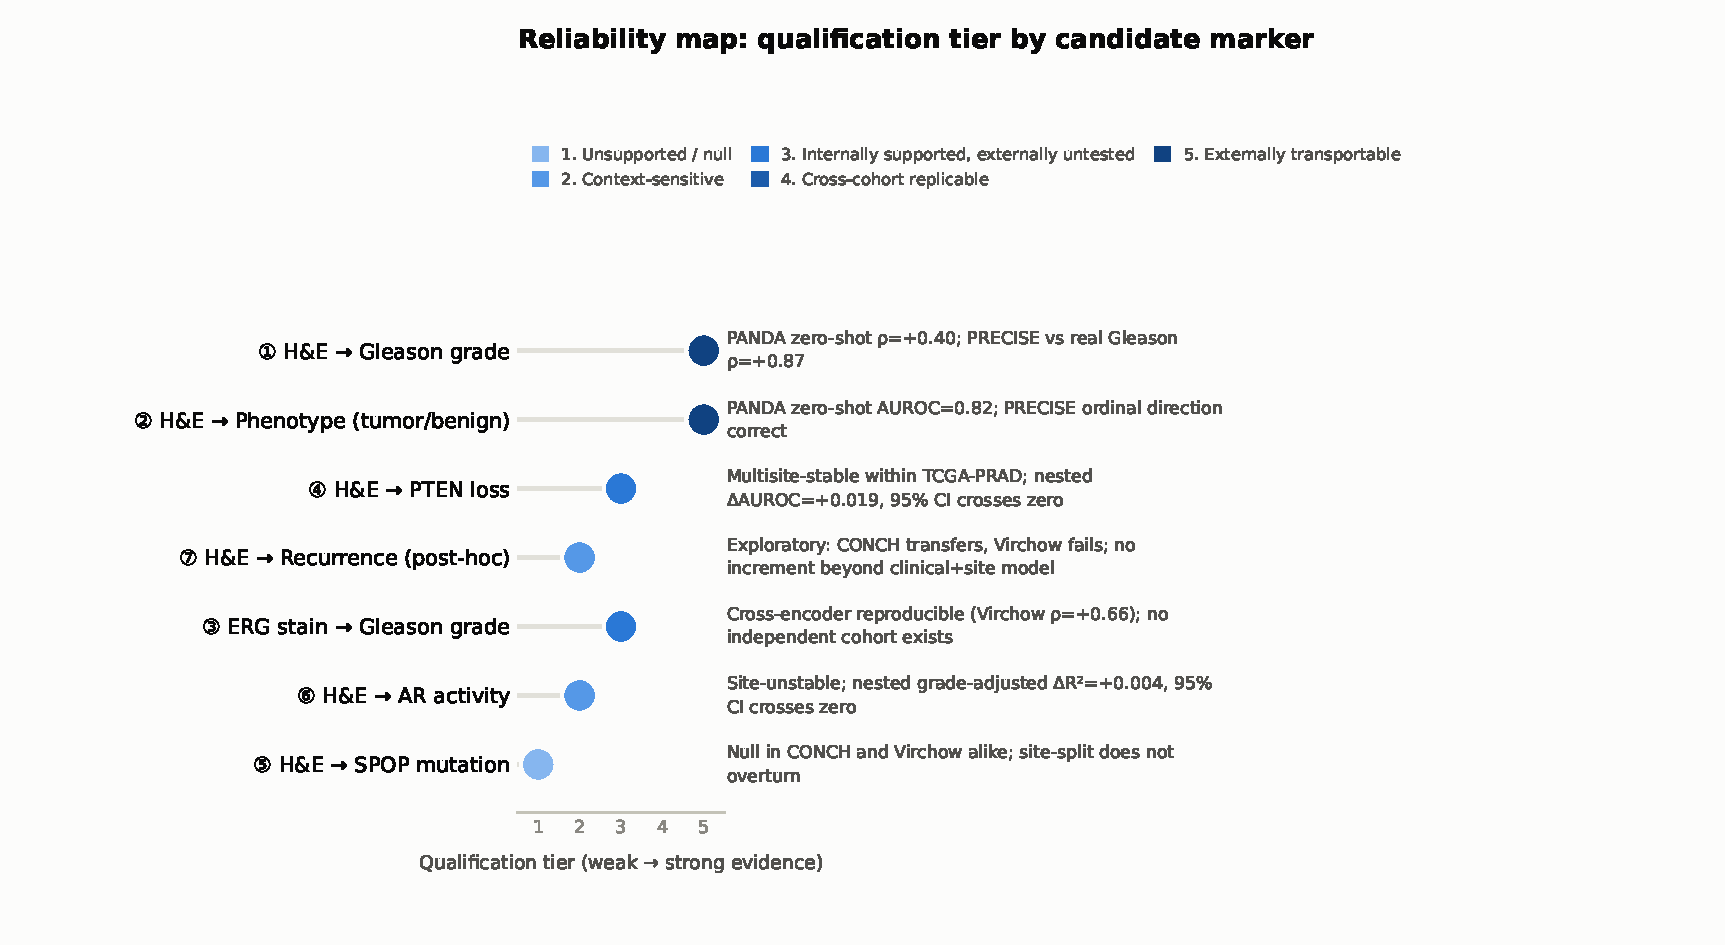
\includegraphics[width=0.92\textwidth]{figures/fig1_reliability_map.pdf}
\caption{Reliability map for the six initially frozen candidates, with marker 7 positioned
descriptively as post-hoc/context-sensitive rather than retrospectively granted a prospective
tier. Key supporting evidence is shown for each marker.}
\label{fig:reliability}
\end{figure}

\begin{table}[htbp]
\centering
\small
\begin{tabular}{lllll}
\toprule
Marker & Target & Training cohort & Patient-level effect & BH-FDR $q$ \\
\midrule
Marker 1 (Grade) & Gleason score & NADT & $\rho=+0.48$ [0.17, 0.71] & 0.0070 \\
Marker 2 (Phenotype) & Tumor/benign & NADT & $\rho=+0.80$ [0.62, 0.91] & $1.6\times10^{-8}$ \\
Marker 3 (ERG$\to$Grade) & Gleason score & NADT (ERG stain) & $\rho=+0.52$ [0.22, 0.75] & 0.0035 \\
Marker 4 (PTEN loss) & CNA loss & TCGA-PRAD & AUROC$=0.63$ [0.56, 0.71] & 0.0035 \\
Marker 5 (SPOP mutation) & Mutation & TCGA-PRAD & AUROC$=0.52$ [0.41, 0.63] & 0.79 (null) \\
Marker 6 (AR activity) & Activity score & TCGA-PRAD & $\rho=+0.19$ [0.07, 0.31] & 0.0052 \\
\bottomrule
\end{tabular}
\caption{Patient-level effect sizes and bootstrap 95\% CIs (2{,}000 resamples), BH-FDR
corrected across the 13 marker hypotheses plus four nested confounder tests (17 total). See Figure~\ref{fig:forest} for the same data as a
forest plot.}
\label{tab:pool}
\end{table}

\begin{figure}[htbp]
\centering
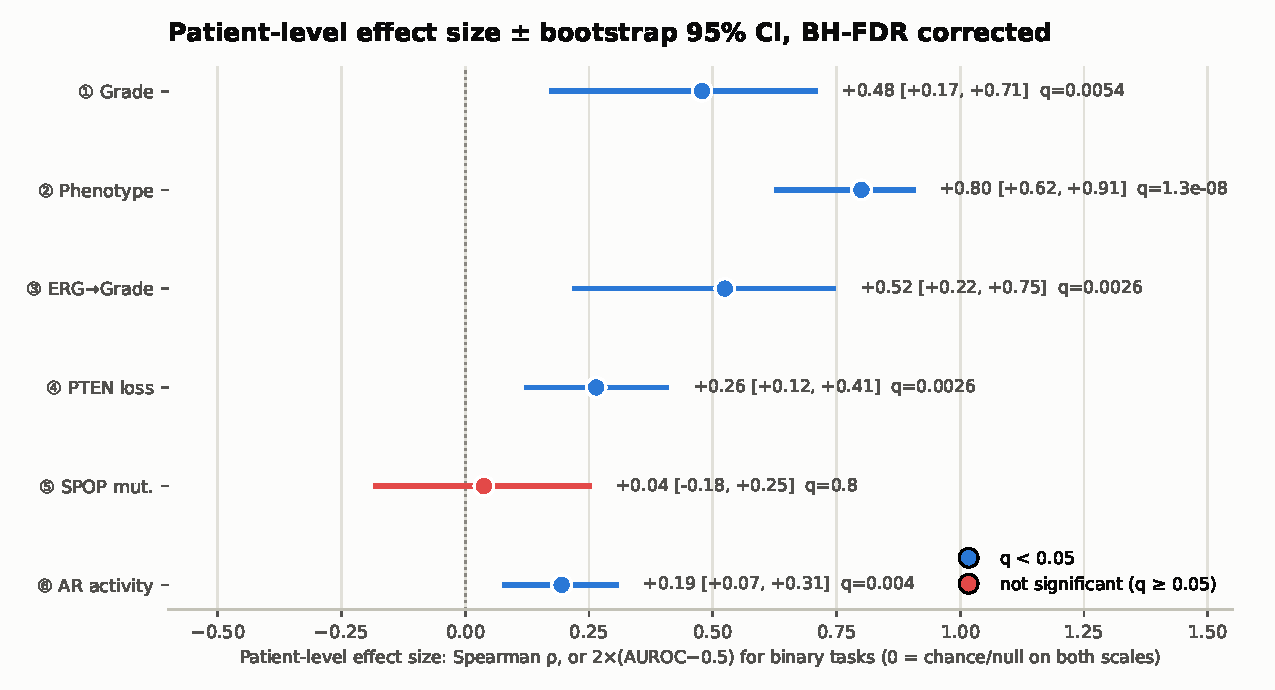
\includegraphics[width=0.75\textwidth]{figures/fig5_forest_plot.pdf}
\caption{Patient-level effect size $\pm$ bootstrap 95\% CI for the six initial frozen-pool
markers. AUROC-based markers are rescaled to $2\times(\mathrm{AUROC}-0.5)$ so that 0
represents chance on the same axis as Spearman $\rho$.}
\label{fig:forest}
\end{figure}

\begin{figure}[htbp]
\centering
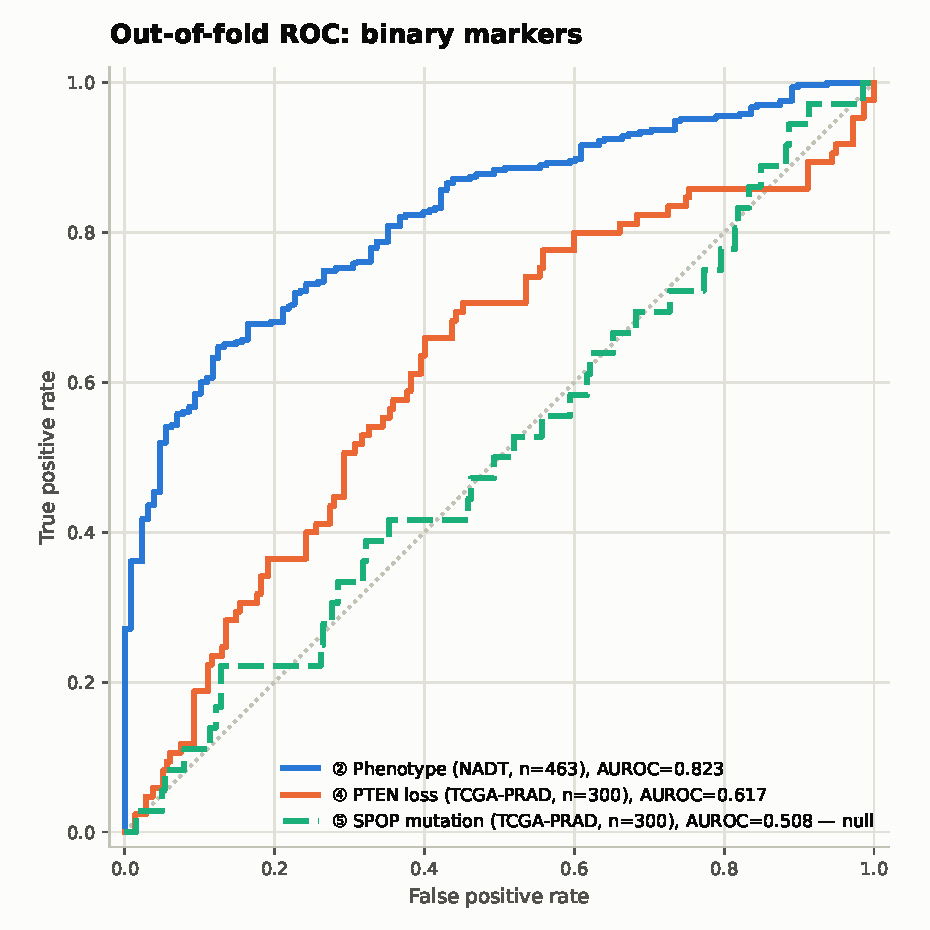
\includegraphics[width=0.85\textwidth]{figures/fig4_roc_curves.pdf}
\caption{Out-of-fold ROC curves for the three binary markers.}
\label{fig:roc}
\end{figure}

\subsection{Cross-encoder replication}

Every marker in the pool was independently re-evaluated with Virchow, a foundation model from
a different organization, architecture, and training corpus than CONCH. Figure~\ref{fig:crossenc}
shows both encoders side by side. Agreement is close for markers 1, 2, 4, and 5 (including the
SPOP null, which replicates independently in Virchow: AUROC$=0.42$). Marker 3 (ERG) is
\emph{stronger} in Virchow. Marker 7 (recurrence) shows the largest divergence and is discussed
separately (Section~\ref{sec:res-marker7}): its CONCH-based zero-shot transfer succeeds where
its Virchow-based counterpart does not, even though Virchow independently carries strong
recurrence signal in both cohorts when refit in-cohort -- an asymmetry in transfer direction,
not in underlying signal.

\begin{figure}[htbp]
\centering
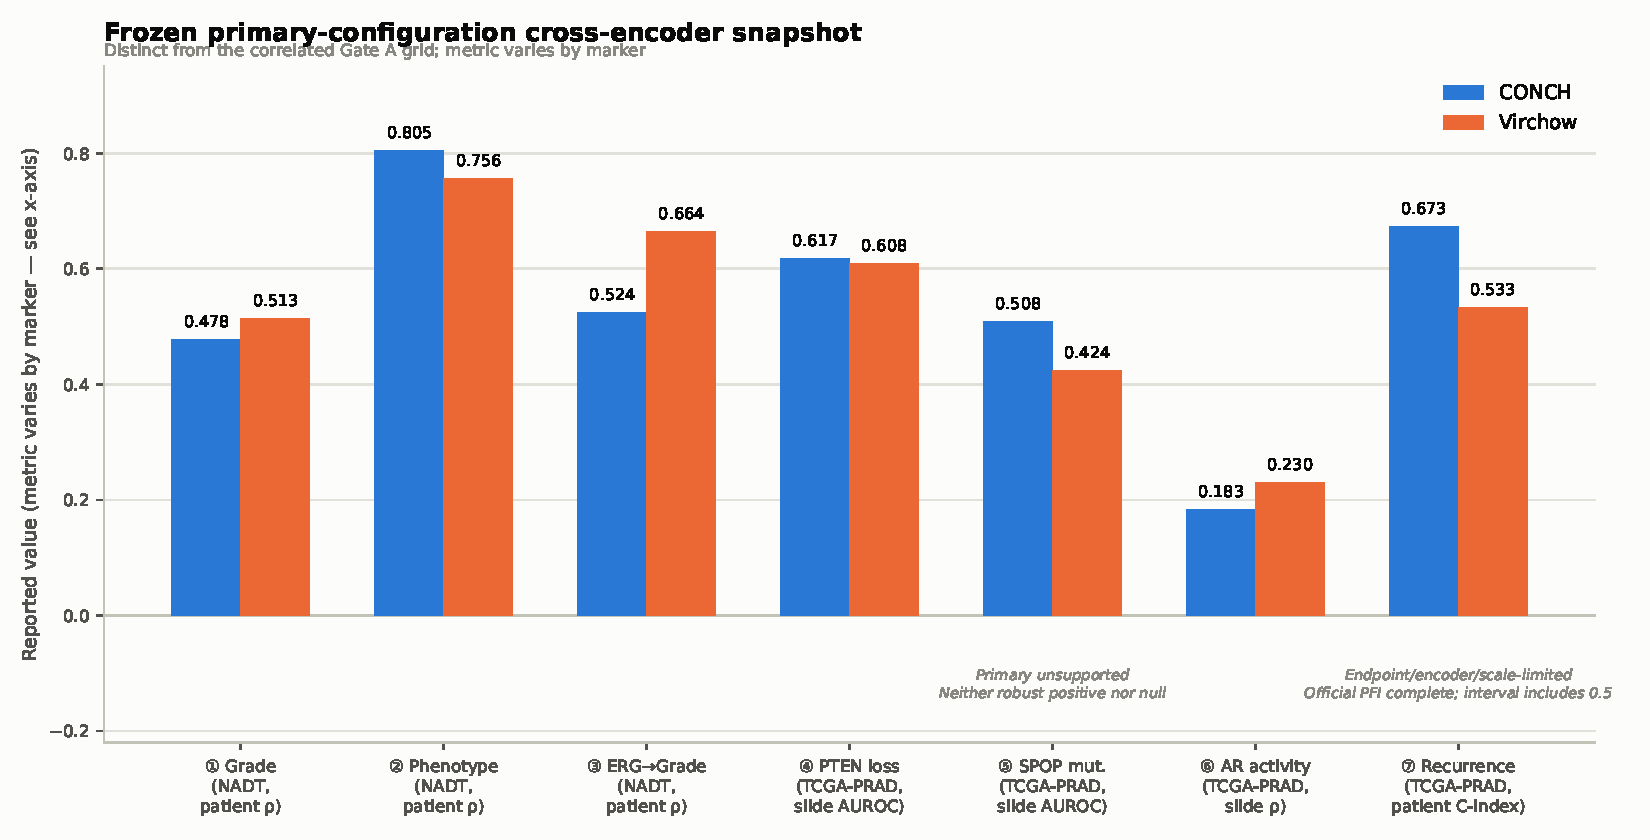
\includegraphics[width=0.92\textwidth]{figures/fig3_conch_vs_virchow.pdf}
\caption{CONCH vs.\ Virchow, all seven markers. Metric type is named per marker (Spearman
$\rho$, AUROC, or C-index); within-marker comparisons are valid, cross-marker magnitude
comparisons are not, since the metric differs.}
\label{fig:crossenc}
\end{figure}

\subsection{Confounder audit: does grade explain everything?}

For markers 4, 6, and (retrospectively) 7, a fully nested clinical-only / image-only / combined
comparison tests held-out incremental value (Table~\ref{tab:confounder},
Figure~\ref{fig:nested-confounder}). The results are materially weaker than the auxiliary
in-sample analyses. PTEN's patient-level $\Delta$AUROC is $+0.019$ (bootstrap 95\% CI
$[-0.025,+0.068]$; fully refit permutation $p=0.203$), and AR's $\Delta R^2$ is $+0.004$
($[-0.036,+0.042]$; $p=0.176$). Neither supports a confident grade-adjusted held-out
increment. The earlier full-cohort LRT/fixed-score permutation results remain positive (PTEN
$p=0.010/0.014$; AR $p=0.003/0.0025$), but are retained only as explicitly in-sample/fixed-score
auxiliary analyses; their disagreement with nested refitting is itself the reason to prefer
the latter.

Marker 7 adds discrimination over grade alone ($\Delta$C-index $+0.062$,
$[+0.008,+0.119]$, refit $p=0.0100$, global BH $q=0.028$), but not over the full clinical
baseline ($+0.002$, $[-0.012,+0.015]$, refit $p=0.305$). The full-baseline permutation has
1{,}998/2{,}000 valid fits; two failed under separation driven by surgical margin and were
excluded rather than assigned favorable null values.

Because this project has repeatedly found CONCH and Virchow disagree on individual results
(most sharply for marker 7's zero-shot transfer, Section~\ref{sec:res-marker7}), a single-encoder
nested result is not yet the strongest available evidence, so we re-ran the same nested
bootstrap pipeline on Virchow embeddings for PTEN and AR (marker 7 was not re-audited here since
its Virchow zero-shot transfer already failed independently). Virchow \emph{converges} with
CONCH rather than diverging: PTEN's held-out $\Delta$AUROC is $+0.035$ (95\% CI
$[-0.013,+0.087]$) and AR's $\Delta R^2$ is $+0.019$ ($[-0.015,+0.051]$) -- both small, both
positive in direction, and both intervals crossing zero, the same qualitative pattern as CONCH.
Agreement between two independently trained encoders on a \emph{weak, uncertain} result is
itself informative: it argues the small nested increment is a property of the underlying
grade--PTEN/AR relationship rather than an artifact specific to CONCH's embedding space.
Figure~\ref{fig:arforest} shows this site effect as a forest plot: leave-one-site-out effect
sizes range from $\rho=-0.13$ (site CH, $n=23$) to $+0.27$ (site KK, $n=31$), each with a
patient-cluster bootstrap 95\% CI (2{,}000 resamples); at these small per-site sample sizes
($n=22$--59) the CIs are wide and every site's CI overlaps zero, so no single site's estimate
is individually significant, but the point estimates' sign flip (negative at CH, consistently
positive at all five other sites) alongside the much tighter, positive pooled estimate
($\rho=+0.195$ [0.07, 0.31], all sites combined via 5-fold internal CV) is the basis for AR's
\emph{context-sensitive} classification -- a real, replicable pooled association whose
site-level stability cannot be confirmed or ruled out from any individual site alone.

\begin{figure}[htbp]
\centering
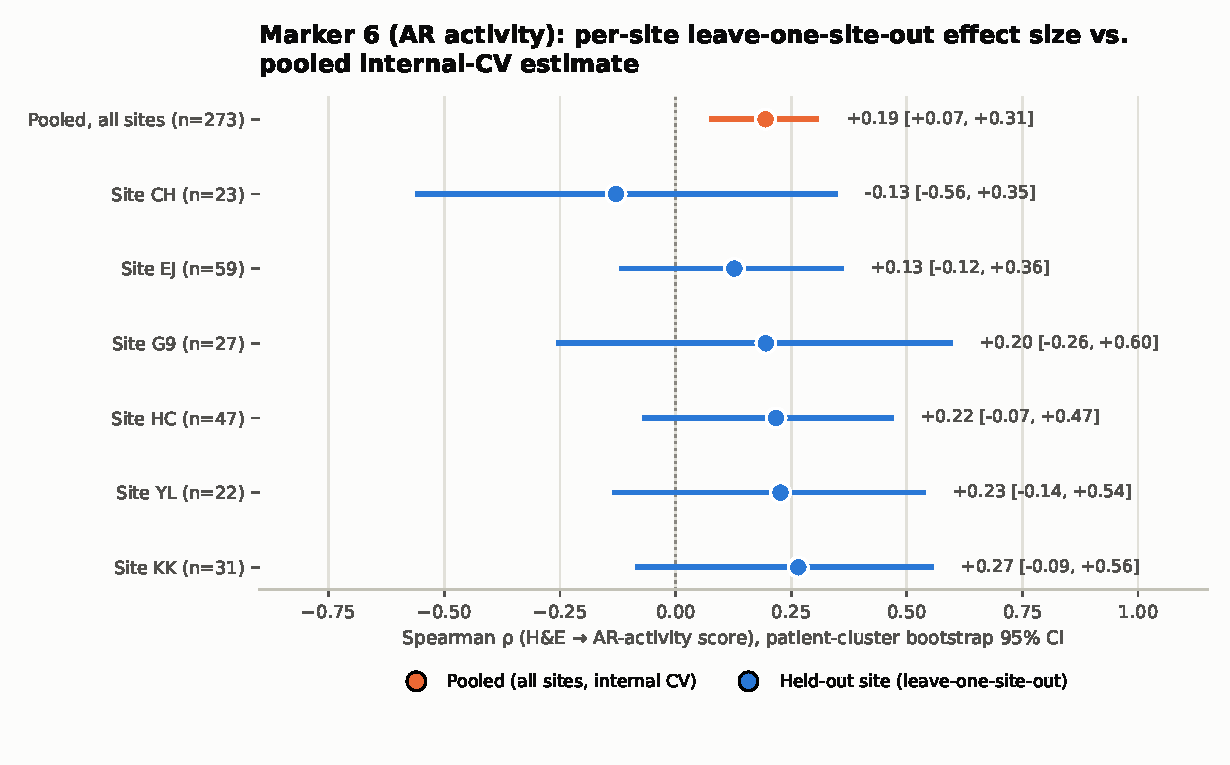
\includegraphics[width=0.85\textwidth]{figures/fig6_ar_site_forest.pdf}
\caption{Marker 6 (AR activity): per-site leave-one-site-out effect size (Spearman $\rho$,
patient-cluster bootstrap 95\% CI, 2{,}000 resamples) vs.\ the pooled all-sites internal-CV
estimate.}
\label{fig:arforest}
\end{figure}

TCGA multi-assay
concordance (PTEN copy-number loss vs.\ mRNA expression vs.\ RPPA protein level, all measured
independently) further supports PTEN as the strongest-triangulated marker in the pool
($p=7.8\times10^{-30}$ CNA-loss vs.\ mRNA, $p=0.001$ CNA-loss vs.\ RPPA), while confirming AR's
three assay layers are correlated but, as previously characterized, not fully independent
(all three are partly RNA-derived).

\begin{table}[htbp]
\centering
\small
\begin{tabular}{lcccccc}
\toprule
Marker & Clinical & Image & Combined & $\Delta$ & 95\% CI & Refit $p$ \\
\midrule
PTEN loss (AUROC) & 0.596 & 0.632 & 0.615 & $+0.019$ & [$-0.025$, 0.068] & 0.203 \\
AR activity ($R^2$) & $-0.003$ & $+0.024$ & $+0.001$ & $+0.004$ & [$-0.036$, 0.042] & 0.176 \\
Recurrence, grade-only (C-index) & 0.645 & 0.664 & 0.707 & $+0.062$ & [0.008, 0.119] & 0.0100 \\
Recurrence, fully adjusted (C-index) & 0.839 & 0.643 & 0.840 & $+0.002$ & [$-0.012$, 0.015] & 0.305 \\
\bottomrule
\end{tabular}
\caption{Nested held-out confounder audit. Metrics are patient-level outer-OOF values;
$\Delta$ is combined minus clinical, with paired patient-bootstrap intervals (2{,}000
resamples). Refit $p$ uses label/event-time permutation within rounded grade strata and
repeats the complete nested pipeline (2{,}000 requested repetitions).}
\label{tab:confounder}
\end{table}

\begin{figure}[htbp]
\centering
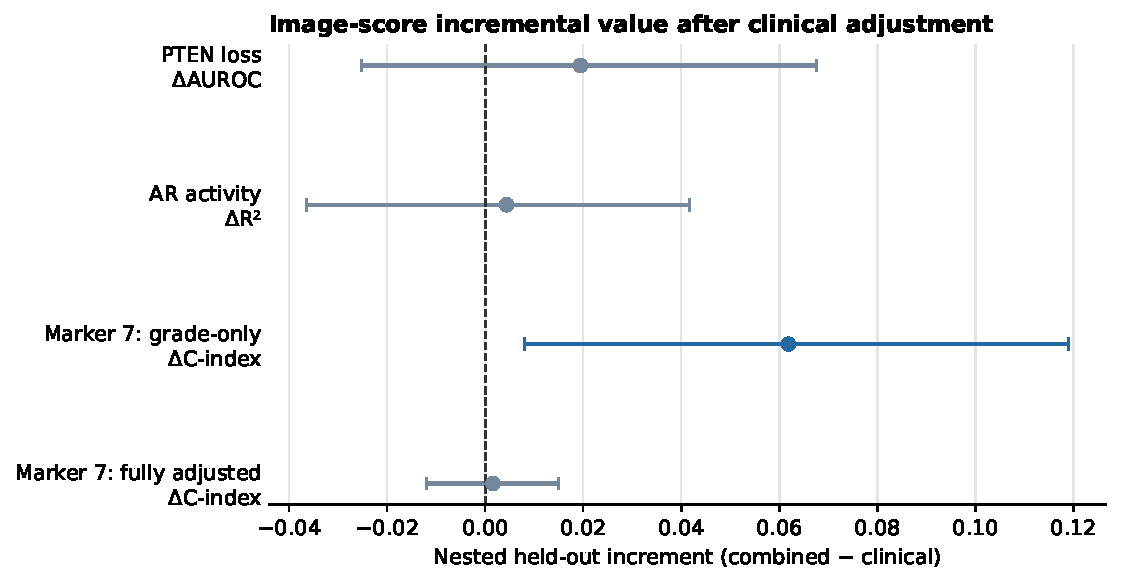
\includegraphics[width=0.78\textwidth]{figures/fig7_nested_confounder.pdf}
\caption{Nested held-out image-score increment over the matched clinical model. Points are
patient-level metric differences and bars are paired patient-bootstrap 95\% confidence
intervals (2{,}000 resamples). Metrics differ by target and are named on the axis labels.}
\label{fig:nested-confounder}
\end{figure}

\subsubsection{Marker 7 against a fully-adjusted clinical baseline}
\label{sec:res-marker7-clinical}

Grade is only one of several standard clinical covariates available for TCGA-PRAD recurrence
modeling. Repeating the confounder audit with a fully-adjusted clinical model (grade, age,
ordinal T-stage, PSA, and binary surgical margin status; Supplementary Table
\ref{tab:supp-marker7-clinical}) on the complete-case subset where all five covariates are
available ($n=153$ of the 270-patient cohort, limited chiefly by PSA, populated for only
167/270 patients in cBioPortal) changes the conclusion: marker7\_risk's added value over the
fully-adjusted clinical model is negligible in nested held-out evaluation ($\Delta$C-index
$=+0.002$, 95\% CI $[-0.012,+0.015]$, refit permutation $p=0.305$), whereas it adds over
grade alone ($+0.062$, $[+0.008,+0.119]$, $p=0.010$; Table~\ref{tab:confounder}). The older
in-sample LRT/fixed-score values ($p=0.215/0.245$ fully adjusted;
$0.0011/0.0015$ grade-only) are auxiliary. Surgical margin status alone is a very
strong predictor in this complete-case subset (recurrence-event rate 67\% among
margin-positive vs.\ 7\% among margin-negative patients, hazard ratio $\approx 13$), and its
inclusion plausibly absorbs much of marker 7's associational signal -- an image-derived score
correlated with visible extraprostatic extension or margin involvement would be expected to
lose independent value once margin status itself enters the model. We cannot fully separate
this explanation from reduced statistical power (57 events at $n=270$ vs.\ 30 events at
$n=153$); we report both the grade-only and fully-adjusted results rather than picking one, and
revise marker 7's characterization accordingly: it adds held-out discrimination beyond a
grade-only model, but not beyond the full standard clinical covariate set; the former should
not be described as general clinical independence.

The sequential held-out hierarchy makes the same point without relying on an in-sample LRT.
M0 (grade) and M1 (grade+age) yield C-indices 0.645 and 0.652 on all 270 patients. Missing PSA
(103/270, 38\%) reduces M2 (grade+PSA+pT) to $n=165$ (C-index 0.687); adding margin in M3
reduces the complete-case cohort to $n=153$, 30 events, and raises C-index to 0.855. M4 adds
site (0.881), while M5 adds marker7 risk and does not improve it (0.879;
$\Delta$C-index $=-0.0024$, paired-bootstrap 95\% CI $[-0.0118,+0.0064]$). Thus the image
score supplies no detectable held-out increment after standard clinical covariates and site.

\subsection{SPOP null: additional robustness checks}

Leave-one-site-out replication (same design as markers 4 and 6 above) is only testable for 3 of
the 6 TCGA-PRAD sites for SPOP, since its low mutation prevalence (12\%, 36/300 slides) leaves
too few positive cases at the other three sites to evaluate AUROC. Across the 3 testable sites,
held-out AUROC is $0.57$--$0.65$ (mean $0.61$) -- nominally above the pooled null estimate
($0.52$), but based on only 3 sites and small held-out counts ($n=31$--59), which is too thin a
basis to overturn the null conclusion on its own; we report it for transparency rather than as
a positive finding. Combined with the independent cross-encoder null (Virchow AUROC$=0.42$), we
also checked whether
the project's standard \texttt{class\_weight="balanced"} choice was itself responsible for the
null, since SPOP mutation prevalence is low (12\%, 36/300 slides). Re-fitting with no class
reweighting gives a nearly identical result (slide AUROC $0.506$ vs.\ $0.508$, patient AUROC
$0.516$ vs.\ $0.519$, both non-significant either way) -- the null is not an artifact of the
class-imbalance handling choice. The balanced patient-level bootstrap interval is
$[0.408,0.627]$, so this design rules out large effects above roughly 0.63 at the 95\% interval
boundary but remains underpowered for modest effects: a Hanley--McNeil normal approximation
places the 80\%-power minimum detectable AUROC at 0.661 (two-sided $\alpha=0.05$). The correct
interpretation is therefore ``no large detectable effect,'' not proof of exact absence.

\subsection{Tile-count and physical-scale sensitivity (markers 4--6)}
\label{sec:res-scale-sensitivity}

To address whether results are sensitive to tile count and physical scale choices (bounded to
one cohort/encoder; a full sweep across every marker/cohort/encoder remains out of scope),
markers 4--6 were evaluated from the same re-embedded, fixed PTEN-status-stratified 90-slide
subsample of TCGA-PRAD across a $3\times3$ grid: tile count $\in\{16,32,64\}$ and physical
scale $\in\{0.44,0.88,1.76\}\,\mu$m/px (half, native, and double this project's standard CONCH
TCGA-PRAD scale), same seed and slide set across all 9 cells so only tile count/scale differ.
An initial version of this grid produced identical results across all three scales at each
tile count -- traced to TCGA-PRAD's SVS files having only 3--4 discrete tiled pyramid levels
(native $\approx\{0.25,1.0,4.0,8.0\}\,\mu$m/px), so a naive nearest-level lookup collapsed all
three intended targets onto the same actual level. This was fixed by combining level choice
with a physically-sized crop window and resize, the same approach already used for PRECISE's
native-resolution mismatch (Methods).

\begin{table}[htbp]
\centering
\small
\begin{tabular}{lccc}
\toprule
Tiles/slide & 0.44 $\mu$m/px & 0.88 $\mu$m/px & 1.76 $\mu$m/px \\
\midrule
16 & 0.488 & 0.598 & 0.643 \\
32 & 0.594 & 0.575 & 0.564 \\
64 & 0.600 & 0.602 & 0.621 \\
\bottomrule
\end{tabular}
\caption{Marker 4 (PTEN loss), patient-level AUROC across the tile-count $\times$ scale grid
($n=85$ patients, fixed 90-slide stratified subsample, single seed).}
\label{tab:scale-sensitivity}
\end{table}

At 16 tiles/slide, patient AUROC ranges from $0.488$ to $0.643$ across the three scales (span
$0.155$) -- a meaningful sensitivity to scale choice at this tile count. At 32 and 64
tiles/slide, the range narrows to $0.564$--$0.594$ and $0.600$--$0.621$ respectively (span
$0.03$ and $0.02$), suggesting that averaging over more tiles attenuates, though does not
eliminate, sensitivity to the exact physical scale within this $4\times$ range. This is a
three-marker, single-seed, subsampled check, not a general claim about scale robustness across
encoders or cohorts -- but within its bounded scope, it is consistent with this project's
existing default of 16--64 tiles/slide, while suggesting the lower end of that range (16 tiles)
is the more scale-sensitive choice and the higher end (64) the more robust one.

Reusing each grid cell's embeddings for AR and SPOP reveals additional setting dependence at
no extra image-encoding cost. AR's patient-level Spearman $\rho$ remains positive in all nine
cells but ranges from $0.114$ to $0.355$ (mean $0.253$, SD $0.078$); its out-of-sample $R^2$
ranges from $-0.074$ to $+0.175$. SPOP patient AUROC ranges from $0.341$ to $0.601$ (mean
$0.471$, SD $0.100$), crossing chance repeatedly without a stable direction. These single-seed
subsample results reinforce AR's context sensitivity and SPOP's lack of a robust effect; they
do not replace the full-cohort primary estimates.

\subsection{LEOPARD: qualification does not guarantee transfer to a downstream outcome}
\label{sec:leopard-results}

Applying the qualified pool's zero-shot markers to LEOPARD's real recurrence outcome, the
three prospectively frozen pools (naive, qualified, all-candidate) all scored \emph{below chance}
(C-index $0.334$--$0.481$; Table~\ref{tab:leopard-survival} reports the full survival-metric
battery). This was not a bug: label alignment was verified exactly
(508/508 case IDs matched via join), and results were unchanged across a wide regularization
sweep. Univariate testing showed every individual marker was null for this specific outcome on
LEOPARD (patient-level C-index/AUROC $0.496$--$0.525$, all $p>0.3$) -- the sub-chance pool
results reflect noise amplification from combining null covariates in a multivariate model
under only 87 events, not a data or pipeline error.

\begin{table}[htbp]
\centering
\small
\begin{tabular}{lccccc}
\toprule
Pool & $n$ & C-index & td-AUROC@5y & IBS & Calibration slope \\
\midrule
Naive (1,2,4,6) & 508 & 0.427 & 0.374 & 0.127 & $-1.10$ \\
Qualified (1,2,4) & 508 & 0.334 & 0.296 & 0.128 & $-4.01$ \\
All-candidate (1,2,4,5,6) & 508 & 0.481 & 0.457 & 0.124 & $+0.33$ \\
\bottomrule
\end{tabular}
\caption{LEOPARD 3-pool zero-shot survival metrics, out-of-fold (5-fold CV). All three pools
score below chance (C-index $<0.5$) and show poorly-behaved calibration slopes (far from the
ideal value of 1, including two pools with the wrong sign), consistent with the pools combining
individually-null markers into an unstable multivariate model rather than any pool containing
usable recurrence signal.}
\label{tab:leopard-survival}
\end{table}

A separate domain-shift diagnostic -- refitting a fresh model directly on LEOPARD's own
embeddings against its own recurrence labels, in-cohort, rather than transferring an existing
probe -- found real signal: C-index $0.598$--$0.661$ across a range of PCA dimensionalities,
stable across random seeds. The zero-shot markers' failure is therefore a transfer failure, not
an absence of recoverable signal in the embedding space -- markers qualified against grade,
phenotype, PTEN, or AR do not automatically carry information about a different downstream
outcome (recurrence), even when that information demonstrably exists in the same embedding
space.

We directly tested whether this in-cohort signal was itself an artifact of observation-time
bias (recently accrued, short-follow-up patients trivially reading as "low risk"). Among
censored patients only, risk score correlated weakly with follow-up duration ($\rho=-0.09$,
$p=0.07$); among the 87 true recurrence events, risk score correlated strongly with time-to-
recurrence ($\rho=-0.42$, $p<10^{-4}$), a pattern specific to genuine prognostic signal. A
landmark analysis restricting evaluation to patients with a definitively known 3- or 5-year
outcome (including early recurrences) preserved discrimination (C-index $0.662$--$0.666$
vs.\ $0.661$ overall) -- inconsistent with an observation-time-bias explanation.

The same diagnostic, repeated with Virchow, reproduced closely (C-index $0.622$--$0.675$,
stable across seeds and the same landmark check), and, most tellingly, CONCH's and Virchow's
independently derived risk scores for the same 508 patients correlated at $\rho=+0.74$
($p=3\times10^{-88}$) -- convergent evidence from two encoders that neither ``discovered''
this signal by chance.

\subsection{Marker 7: post-hoc discovery, external validation, and an encoder asymmetry}
\label{sec:res-marker7}

The LEOPARD-fitted recurrence model transfers zero-shot to TCGA-PRAD (using recurrence-style
labels reconstructed from GDC's \texttt{follow\_ups.disease\_response} field, since a
pre-existing label file could not be traced to a generating script and failed a spot check):
C-index$=0.673$, matching or exceeding LEOPARD's own in-cohort performance, robust to the same
landmark analysis (3-year C-index$=0.675$, 5-year $=0.647$). Beyond C-index and td-AUROC, the
same zero-shot transfer has an integrated Brier score of $0.124$ (over 0.5--10 years) and a
calibration slope of $0.53$ (1.0 = perfect calibration; a slope below 1 indicates the
LEOPARD-fitted risk score is directionally correct but over-dispersed on TCGA-PRAD, consistent
with applying coefficients fitted on one cohort's absolute risk scale to a different cohort
without recalibration), and marker7\_risk corresponds to a hazard ratio of $1.71$ per unit
increase (95\% CI $[1.34, 2.18]$) in a univariate Cox model. This is exploratory cross-cohort
directional evidence, not a prospectively tiered validation: it uses a coarser,
clinical-assessment-based outcome than LEOPARD's PSA-based one and was discovered only after
seeing the LEOPARD results. The confounder audit above (Table~\ref{tab:confounder}) shows a
held-out increment over grade alone, though not over the fully-adjusted clinical covariate set
(Section~\ref{sec:res-marker7-clinical}).

The same transfer, repeated with Virchow (first at Virchow's native tile scale, then
re-embedded at LEOPARD's tile scale to rule out a scale-mismatch explanation) failed both
times (C-index $0.545$ and $0.533$). Yet Virchow's own in-cohort fit on TCGA-PRAD is, if
anything, stronger than CONCH's (C-index up to $0.795$ vs.\ $0.72$--$0.74$) -- so the failure
is not an absence of Virchow signal, but a genuine encoder-dependent transfer-direction
mismatch, one further instance of the general pitfall that different encoders' embedding
spaces organize signal differently even when each independently contains it.

\subsection{Benchmarking the reconstructed recurrence label against standard TCGA endpoints}
\label{sec:res-label-benchmark}

Because marker 7's TCGA-PRAD label is reconstructed rather than a standard endpoint, we
benchmark it directly against TCGA's own standardized TCGA-CDR endpoints (Liu et al.\ 2018:
progression-free survival, PFS, and disease-free survival, DFS), obtained from cBioPortal study
\texttt{prad\_tcga\_pan\_can\_atlas\_2018}, for the 270-patient embedded cohort. Event-status
agreement is substantial but not perfect: 87.0\% raw agreement with PFS\_STATUS (Cohen's
$\kappa=0.57$, $n=270$) and 93.2\% with DFS\_STATUS (Cohen's $\kappa=0.52$, $n=192$; DFS is
only defined for patients with curative-intent treatment and no prior malignancy, per TCGA-CDR
convention, hence the smaller $n$). Our label flags more patients as having recurred than PFS
does (confusion matrix: 25 patients we label as events that PFS calls censored, vs.\ 10 in the
reverse direction), consistent with our label's coarser, clinical-assessment-based definition
(persistent or recurrent tumor at any follow-up visit) capturing a broader construct than PFS's
progression-specific one. Follow-up time itself agrees closely with both standard endpoints
(Spearman $\rho=+0.85$ vs.\ PFS\_MONTHS, $+0.95$ vs.\ DFS\_MONTHS, both $p<10^{-75}$).

Re-scoring marker 7's zero-shot transfer using PFS or DFS directly as the outcome, instead of
our reconstructed label, gives C-index$=0.586$ (td-AUROC@5y$=0.610$, $n=270$, 42 events) against
PFS and C-index$=0.605$ (td-AUROC@5y$=0.592$, $n=192$, only 11 events) against DFS -- both
above chance and directionally consistent with the original C-index$=0.673$ using our
reconstructed label, but visibly attenuated, particularly against PFS's stricter
progression-only definition. We read this as a partial validation and a partial caveat
together: marker 7's zero-shot signal is not an artifact specific to our label reconstruction
(it transfers, above chance, to TCGA's own standardized endpoint), but the original
C-index$=0.673$ headline number is somewhat label-definition-specific, and the more standard
PFS endpoint yields a more modest, though still meaningfully above-chance, transfer.

The stricter persistent-disease-excluding endpoint changes the estimand sharply. Of 111 events
in all 493 labeled TCGA-PRAD cases, only 11 occur strictly after an earlier documented
tumor-free visit; 100 first/only or same-day with-tumor observations are classified as
persistent/indeterminate and excluded. Within the embedded cohort this leaves $n=220$ and
only 7 events. Direction is retained (C-index $0.655$, 5-year td-AUROC $0.566$), but seven events are far too few for a strong
recurrence-validation claim. Across the original endpoint, td-AUROC declines from $0.740$ at
1 year to $0.636$ at 5 years (mean 1--5-year AUC $0.714$), and risk-quintile calibration shows
substantial overprediction, consistent with the calibration slope below one. We therefore
characterize marker 7 as an endpoint-sensitive, post-hoc exploratory transfer rather than a
clinically incremental recurrence marker.

\begin{figure}[htbp]
\centering
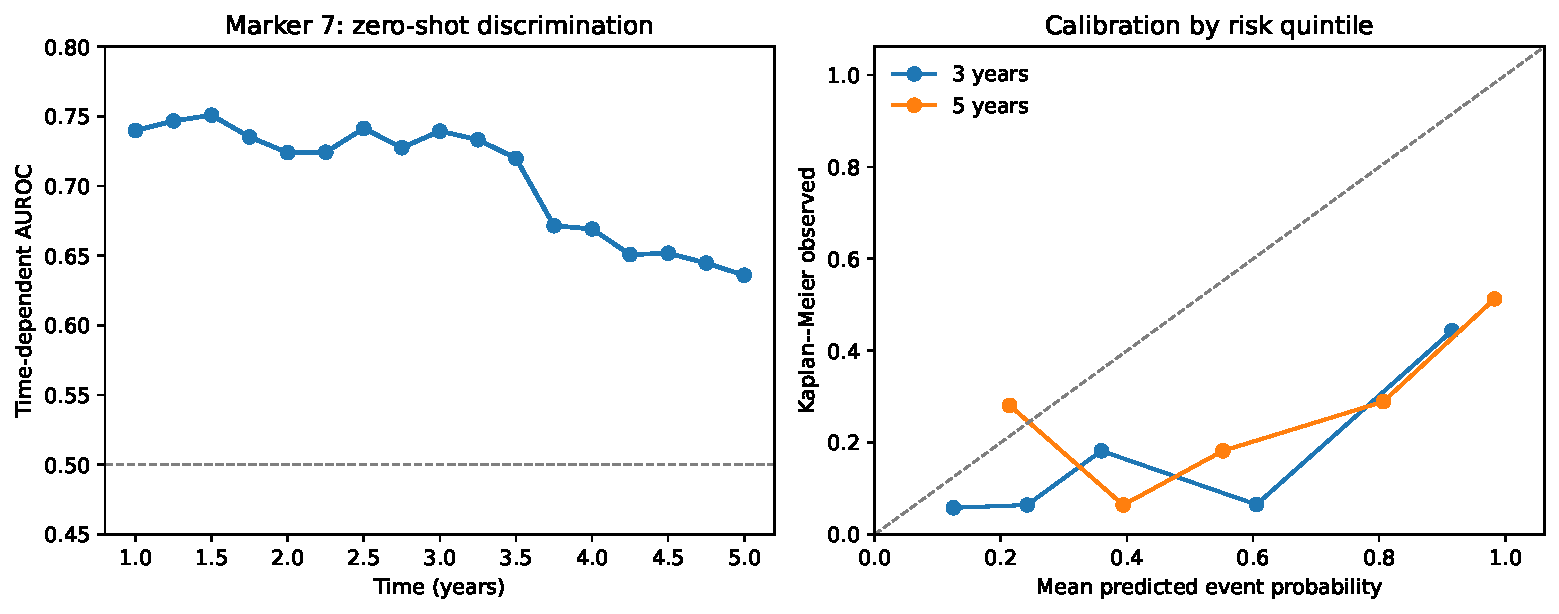
\includegraphics[width=0.90\textwidth]{figures/fig_marker7_survival_curves.pdf}
\caption{Marker 7 zero-shot survival sensitivity on TCGA-PRAD. Left: time-dependent AUROC
from 1--5 years. Right: predicted vs.\ Kaplan--Meier-observed 3- and 5-year event probability
by predicted-risk quintile. Discrimination remains above chance while absolute risk is
substantially overpredicted without recalibration.}
\label{fig:marker7-survival-curves}
\end{figure}

\subsection{PRECISE: spatial face-validity and real-Gleason external validation}

Tile-level scoring against PRECISE's pixel-level expert annotations (Figure~\ref{fig:m1ext}a
scatter; annotation regions are small relative to standard tiling, requiring a
$150\,\mu$m window rather than the $\approx 394\,\mu$m used elsewhere to obtain any
qualifying benign-gland tiles) shows marker 1 in a clean monotonic order across tissue class:
benign gland (mean predicted grade 5.2) $\ll$ stroma (7.7) $<$ tumor (8.7) -- exactly the
expected pattern, since Gleason grading does not conceptually apply to benign tissue.

\textbf{Aggregation unit.} All PRECISE scoring is aggregated per imaging session (25 patients,
27 sessions total -- one patient contributes three sessions, all others one each; ``image'' in
this section always means one session, i.e.\ \texttt{sub-XX\_ses-YY}, not one patient). Averaged
per session and compared against real pathologist-assigned Gleason score, marker 1 achieves
Spearman $\rho=+0.87$ ($p=7.6\times10^{-6}$, $n=17$ sessions), zero-shot, on a cohort never used
in any training step. As a robustness check against over-counting patients with multiple
sessions: all 17 sessions in this specific real-Gleason comparison happen to come from 17
distinct patients (the one multi-session patient's other two sessions either lacked a
comparable Gleason label or no qualifying tumor tile), so the session-level and patient-level
aggregations of this particular result are numerically identical ($\rho=+0.87$ either way) --
the correlation is not an artifact of any patient being over-represented. Marker 2 (phenotype)
preserves the correct ordinal direction (tumor $>$ benign $>$ stroma by median tumor-probability)
but saturates near ceiling at this fine spatial scale, a granularity mismatch with NADT's
coarser whole-slide training signal that we report as an honest limitation rather than a
further positive result.

\subsection{QWK and comparison to literature}

Table~\ref{fig:m1ext}b converts marker 1's continuous predictions to quadratic weighted kappa
(QWK) for direct comparison with literature figures reported in that unit. Zero-shot QWK
($0.26$--$0.39$) is well below fully supervised PANDA-challenge-winner performance ($\approx
0.86$), an expected gap given this study evaluates a frozen general-purpose embedding with a
linear probe and zero retraining against purpose-built, massively supervised models -- a gap
consistent with, not contradicting, this study's positioning as a reproducibility and
transportability audit rather than a grading-accuracy benchmark. PRECISE's real-Gleason QWK
($0.788$) approaches the supervised benchmark but is based on only 17 images and should not be
over-interpreted as a comparable-scale result.

\begin{figure}[htbp]
\centering
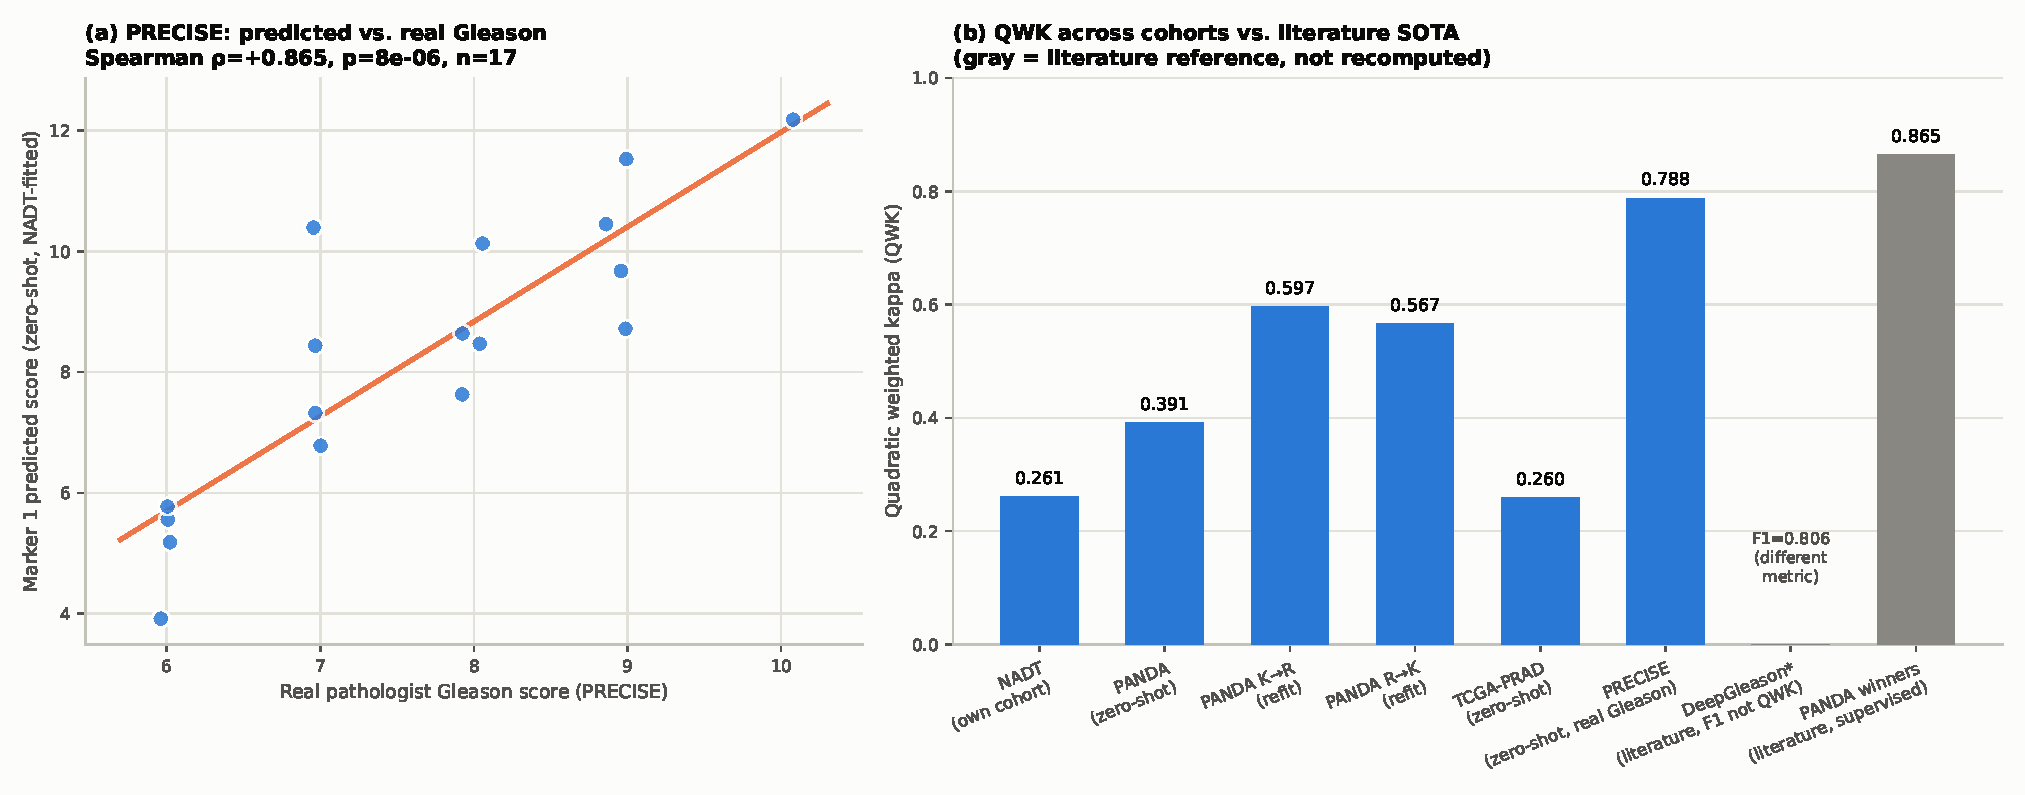
\includegraphics[width=0.98\textwidth]{figures/fig2_marker1_external.pdf}
\caption{(a) Marker 1 predicted vs.\ real pathologist Gleason score on PRECISE. (b) QWK across
all evaluated cohorts and two literature reference points (gray).}
\label{fig:m1ext}
\end{figure}
